\chapter{الأزهار والثمار والبذور}\label{ch:g3:flowers-fruits-seeds}

في نيسان تبيضّ شجرة الكرز بالزهر؛ وفي حزيران تتدلى بالكرز. فأين
ذهبت الأزهار --- ومن أين جاءت \omterm{prop:g3:flowers-fruits-seeds:transform}{الثمار}؟ والجواب واحد من أجمل
التحولات في العالم الحي: \omterm{def:g3:flowers-fruits-seeds:parts}{الزهرة} لا تختفي، بل \emph{تصير} \omterm{prop:g3:flowers-fruits-seeds:transform}{الثمرة}.

\section{نظرة داخل الزهرة}

\begin{definition}[أجزاء الزهرة]\label{def:g3:flowers-fruits-seeds:parts}
\emph{الزهرة}\index{زهرة} هي جزء \omterm{def:g1:plants-around-us:plant}{النبات} الذي سيصنع \omterm{def:g2:from-seed-to-plant:seed}{البذور}. ومن
الخارج إلى الداخل:
\begin{enumerate}
  \item \emph{البتلات}\index{بتلة}، وهي ملونة عطرة، تجذب \omterm{prop:g3:sorting-living-things:groups}{الحشرات}
        الزائرة؛
  \item و\emph{الأسدية}\index{سداة}، وهي سويقات رفيعة يغبّرها
        \emph{حبوب اللقاح}\index{حبوب اللقاح}، وهي مسحوق أصفر
        ناعم؛
  \item و\emph{المدقة}\index{مدقة} في الوسط تمامًا، وهي قارورة
        صغيرة؛ وفي عمقها تقع \omterm{def:g2:from-seed-to-plant:seed}{بذور} الزهرة المستقبلية.
\end{enumerate}
\end{definition}

\begin{omfigure}
\begin{tikzpicture}
  \node[anchor=south west, inner sep=0] (img) at (0,0)
    {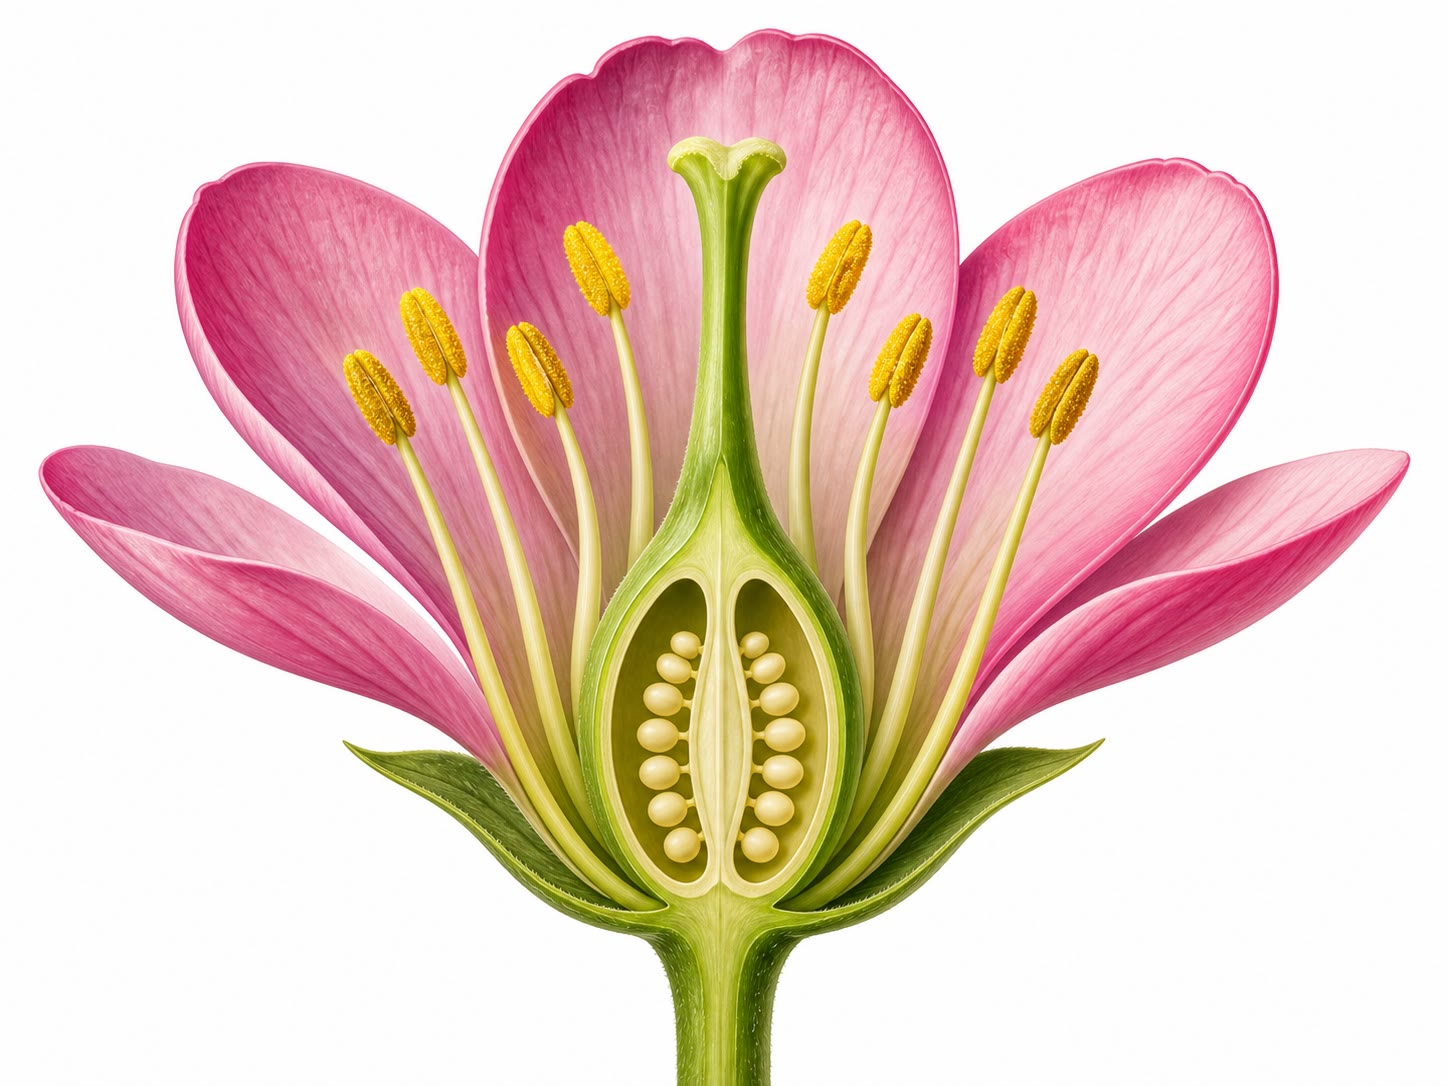
\includegraphics[width=0.6\linewidth]{images/book1/ai/fig-flower-cutaway.jpg}};
  \begin{scope}[x={(img.south east)}, y={(img.north west)},
      every node/.style={font=\small}]
    \draw[omDef, thick] (0.82,0.80) -- (0.93,0.90) node[above] {بتلة};
    \draw[omDef, thick] (0.72,0.68) -- (1.03,0.66)
      node[right, align=left] {سداة مغبَّرة\\ بحبوب اللقاح};
    \draw[omDef, thick] (0.56,0.36) -- (1.03,0.34)
      node[right, align=left] {مدقة: البذور\\ المستقبلية في داخلها};
    \draw[omDef, thick] (0.505,0.05) -- (0.66,0.04) node[right] {ساق};
  \end{scope}
\end{tikzpicture}

{\small داخل \omterm{def:g3:flowers-fruits-seeds:parts}{زهرة} مقطوعة نصفين: \omterm{def:g3:flowers-fruits-seeds:parts}{بتلات} حولها، \omterm{def:g3:flowers-fruits-seeds:parts}{وأسدية} حاملة \omterm{def:g3:flowers-fruits-seeds:parts}{لحبوب
اللقاح}، \omterm{def:g3:flowers-fruits-seeds:parts}{ومدقة} في الوسط فيها \omterm{def:g2:from-seed-to-plant:seed}{البذور} المستقبلية.}
\end{omfigure}

\begin{example}[تشريح زهرة خزامى]\label{ex:g3:flowers-fruits-seeds:tulip}
افتح \omterm{def:g3:flowers-fruits-seeds:parts}{زهرة} خزامى ذابلة برفق، بتلةً \omterm{def:g3:flowers-fruits-seeds:parts}{بتلة}. ففي داخلها تقف \omterm{def:g3:flowers-fruits-seeds:parts}{الأسدية} ---
امسح واحدة على إصبعك فتترك غبار لقاح أصفر --- وفي الوسط \omterm{def:g3:flowers-fruits-seeds:parts}{المدقة}
الخضراء السمينة. واقطع \omterm{def:g3:flowers-fruits-seeds:parts}{المدقة} عرضًا (وهذا عمل سكين يقوم به كبير)
فإذا هي هناك: صفوف من \omterm{def:g2:from-seed-to-plant:seed}{بذور} مستقبلية شاحبة صغيرة.
\end{example}

\section{من الزهرة إلى الثمرة}

\begin{proposition}[التأبير ثم التحول]\label{prop:g3:flowers-fruits-seeds:transform}
لكي يبدأ \omterm{def:g2:animals-grow-up:metamorphosis}{التحول}، لا بد أن تبلغ \omterm{def:g3:flowers-fruits-seeds:parts}{حبوب اللقاح} \omterm{def:g3:flowers-fruits-seeds:parts}{المدقة} --- وتلك الخطوة
هي \emph{التأبير}\index{تأبير}. والنحل \omterm{prop:g3:sorting-living-things:groups}{والحشرات} الأخرى تقوم بأكثر
النقل، وهي مغبَّرة \omterm{def:g3:flowers-fruits-seeds:parts}{بحبوب اللقاح} وهي تشرب من \omterm{def:g3:flowers-fruits-seeds:parts}{زهرة} إلى \omterm{def:g3:flowers-fruits-seeds:parts}{زهرة}؛ والريح
تقوم ببعضه أيضًا. وبعد التأبير:
\begin{itemize}
  \item تذبل \omterm{def:g3:flowers-fruits-seeds:parts}{البتلات} \omterm{def:g3:flowers-fruits-seeds:parts}{والأسدية} وتسقط، وقد انتهى عملها؛
  \item وتنتفخ \omterm{def:g3:flowers-fruits-seeds:parts}{المدقة} فتصير \emph{الثمرة}\index{ثمرة}؛
  \item وتصير \omterm{def:g2:from-seed-to-plant:seed}{البذور} المستقبلية داخلها \emph{بذورًا}\index{بذرة}.
\end{itemize}
\omterm{prop:g3:flowers-fruits-seeds:transform}{والثمرة} \omterm{def:g3:flowers-fruits-seeds:parts}{مدقة} متحولة، وكل \omterm{prop:g3:flowers-fruits-seeds:transform}{ثمرة} حقيقية تحمل بذورًا.
\end{proposition}
\admitted

\begin{example}[مشاهدة كرزة واحدة تتكوّن]\label{ex:g3:flowers-fruits-seeds:cherry}
تتبّع \omterm{def:g3:flowers-fruits-seeds:parts}{زهرة} كرز واحدة. في نيسان: \omterm{def:g3:flowers-fruits-seeds:parts}{بتلات} بيضاء ونحل يدندن. وفي أيار:
\omterm{def:g3:flowers-fruits-seeds:parts}{البتلات} تتساقط كالثلج؛ ومكان كل \omterm{def:g3:flowers-fruits-seeds:parts}{زهرة} كرة خضراء صغيرة --- هي \omterm{def:g3:flowers-fruits-seeds:parts}{المدقة}
المنتفخة. وفي حزيران: الكرة قد احمرّت وحلت --- كرزة، في داخلها
النواة (بذرتها). \omterm{def:g3:flowers-fruits-seeds:parts}{فالزهرة} لم تسقط؛ وإنما سقطت بتلاتها.
\end{example}

\begin{remark}[لا نحل، فلا كرز]\label{rem:g3:flowers-fruits-seeds:bees}
يرحّب مزارعو الكرز بخلايا النحّالين في بساتينهم --- فمن غير زيارات
\omterm{prop:g3:sorting-living-things:groups}{الحشرات} تبقى أكثر الأزهار غير مؤبَّرة وتسقط من غير أن تصير ثمرًا
أبدًا. والنحلة لا تسرق من \omterm{def:g3:flowers-fruits-seeds:parts}{الزهرة}؛ بل \omterm{def:g3:flowers-fruits-seeds:parts}{الزهرة} والنحلة تغذّي إحداهما
الأخرى: رحيق للنحلة، وتوصيل \omterm{def:g3:flowers-fruits-seeds:parts}{لحبوب اللقاح} \omterm{def:g1:plants-around-us:plant}{للنبات}.
\end{remark}

\begin{omfigure}
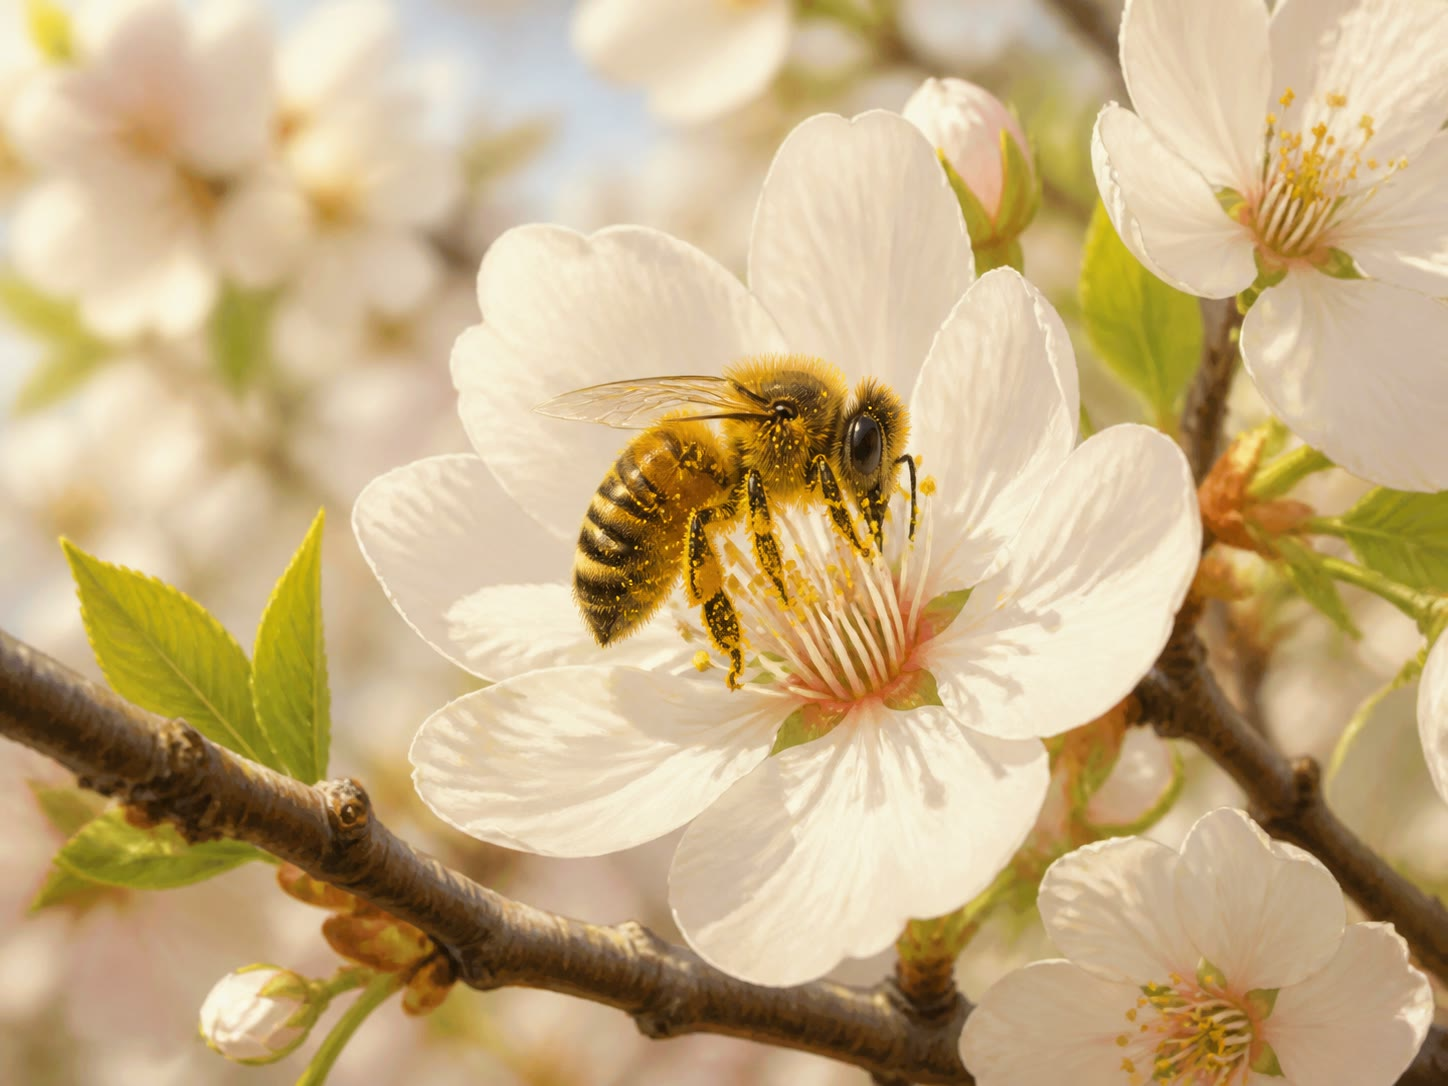
\includegraphics[width=0.58\linewidth]{images/book1/ai/g3-flowers-bee.jpg}

{\small التأبير وهو يجري: نحلة في عمق \omterm{def:g3:flowers-fruits-seeds:parts}{زهرة} كرز، مغبَّرة \omterm{def:g3:flowers-fruits-seeds:parts}{بحبوب
اللقاح} التي ستوصلها إلى \omterm{def:g3:flowers-fruits-seeds:parts}{الزهرة} التالية.}
\end{omfigure}

\section{ثمرة أم غير ثمرة؟}

\begin{method}[اختبار البذور]\label{met:g3:flowers-fruits-seeds:test}
لتقرر أكان شيء من عند الخضريّ \omterm{prop:g3:flowers-fruits-seeds:transform}{ثمرة} بمعنى علماء الأحياء:
\begin{enumerate}
  \item اقطعه؛
  \item وابحث عن \omterm{def:g2:from-seed-to-plant:seed}{بذور} (أو عن نواة، وهي \omterm{def:g2:from-seed-to-plant:seed}{بذرة} في قشرة صلبة)؛
  \item فإن كانت فيه \omterm{def:g2:from-seed-to-plant:seed}{بذور} فقد نما من \omterm{def:g3:flowers-fruits-seeds:parts}{مدقة} \omterm{def:g3:flowers-fruits-seeds:parts}{زهرة}: إنه \omterm{prop:g3:flowers-fruits-seeds:transform}{ثمرة}. وإن لم
        تكن فيه \omterm{def:g2:from-seed-to-plant:seed}{بذور} البتة فهو جزء آخر من \omterm{def:g1:plants-around-us:plant}{النبات}: \omterm{def:g1:plants-around-us:parts}{جذر}، أو \omterm{def:g1:plants-around-us:parts}{ساق}، أو
        \omterm{def:g1:plants-around-us:parts}{ورقة}.
\end{enumerate}
\end{method}

\begin{example}[مفاجآت عند الخضريّ]\label{ex:g3:flowers-fruits-seeds:surprise}
اختبار \omterm{def:g2:from-seed-to-plant:seed}{البذور} يخبئ مفاجآت. الطماطم: ملأى \omterm{def:g2:from-seed-to-plant:seed}{بالبذور} --- \omterm{prop:g3:flowers-fruits-seeds:transform}{ثمرة}، مهما
قال طبق السلطة. والخيار والكوسا: \omterm{def:g2:from-seed-to-plant:seed}{بذور} --- ثمرتان. وقرن الفاصولياء
الخضراء: \omterm{def:g2:from-seed-to-plant:seed}{بذور} في صف --- \omterm{prop:g3:flowers-fruits-seeds:transform}{ثمرة}. والجزرة: لا \omterm{def:g2:from-seed-to-plant:seed}{بذور} ---
\omterm{def:g1:plants-around-us:parts}{جذر} (وقد خمّنه \cref{exo:g1:plants-around-us:10}). والخس: لا
\omterm{def:g2:from-seed-to-plant:seed}{بذور} --- \omterm{def:g1:plants-around-us:parts}{أوراق}. والبطاطا: لا \omterm{def:g2:from-seed-to-plant:seed}{بذور} --- \omterm{def:g1:plants-around-us:parts}{ساق} منتفخة تحت الأرض.
\end{example}

\begin{remark}[كلام المطبخ وكلام العلم]\label{rem:g3:flowers-fruits-seeds:words}
في المطبخ تعني ``الفاكهة'' ما كان حلوًا، وتعني ``الخضرة'' ما كان
مالحًا --- وهذا مفيد لتدبير الحلوى، لا فائدة منه في \omterm{def:g1:living-or-not:living}{علم الأحياء}.
أما كلمة عالم الأحياء فتتبع اختبار \omterm{def:g2:from-seed-to-plant:seed}{البذور}. وكلا المعجمين حسن، ما
دمت تعرف بأيهما تتكلم.
\end{remark}

\section{تمارين}

\begin{exercise}[$\star$]\label{exo:g3:flowers-fruits-seeds:1}
سمِّ أجزاء \omterm{def:g3:flowers-fruits-seeds:parts}{الزهرة} من الخارج إلى الداخل، مع عمل كل جزء.
\end{exercise}

\begin{exercise}[$\star$]\label{exo:g3:flowers-fruits-seeds:2}
ما \omterm{def:g3:flowers-fruits-seeds:parts}{حبوب اللقاح}، وأين توجد؟ وما التأبير؟
\end{exercise}

\begin{exercise}[$\star$]\label{exo:g3:flowers-fruits-seeds:3}
بعد التأبير، ماذا يصير من: (أ) \omterm{def:g3:flowers-fruits-seeds:parts}{البتلات}؟ (ب) \omterm{def:g3:flowers-fruits-seeds:parts}{المدقة}؟ (ج) \omterm{def:g2:from-seed-to-plant:seed}{البذور}
المستقبلية في داخلها؟
\end{exercise}

\begin{exercise}[$\star$]\label{exo:g3:flowers-fruits-seeds:4}
أعد حكاية كرزة واحدة، من \omterm{def:g3:flowers-fruits-seeds:parts}{الزهرة} البيضاء إلى \omterm{prop:g3:flowers-fruits-seeds:transform}{الثمرة} الحمراء، في
ثلاث خطوات مؤرخة.
\end{exercise}

\begin{exercise}[$\star$]\label{exo:g3:flowers-fruits-seeds:5}
لماذا يرحّب مزارعو الكرز بخلايا النحل في البستان؟
\end{exercise}

\begin{exercise}[$\star$]\label{exo:g3:flowers-fruits-seeds:6}
اذكر اختبار \omterm{def:g2:from-seed-to-plant:seed}{البذور}، وطبّقه على الطماطم وعلى الجزرة.
\end{exercise}

\begin{exercise}[$\star$]\label{exo:g3:flowers-fruits-seeds:7}
\omterm{prop:g3:flowers-fruits-seeds:transform}{ثمرة} أم لا، باختبار \omterm{def:g2:from-seed-to-plant:seed}{البذور}: الخيار، والخس، وقرن الفاصولياء
الخضراء، والبطاطا؟
\end{exercise}

\begin{exercise}[$\star$]\label{exo:g3:flowers-fruits-seeds:8}
جرّب: اقطع في البيت ثلاثة أشياء من المطبخ وطبّق اختبار \omterm{def:g2:from-seed-to-plant:seed}{البذور} على
كل واحد. أيها فاجأك؟
\end{exercise}

\begin{exercise}[$\star\star$]\label{exo:g3:flowers-fruits-seeds:9}
يقتل صقيع متأخر كل زهر شجرة الخوخ في نيسان. فما حصاد حزيران،
ولماذا؟ استعمل \cref{prop:g3:flowers-fruits-seeds:transform}.
\end{exercise}

\begin{exercise}[$\star\star$]\label{exo:g3:flowers-fruits-seeds:10}
``التفاحة تنمو لنجد ما نأكله لذيذًا.'' فما غاية التفاحة حقًّا من
وجهة نظر شجرة التفاح؟ وما الذي يقع في قلبها، وإلام يمكن أن يصير كل
واحد منه؟ (تذكّر \cref{ch:g2:from-seed-to-plant}.)
\end{exercise}
